%51741c53-3c67-41d1-9349-9a6a3686d422
% Although we try to provide a template that completely
% matches the corresponding assignment, we do expect you
% to check that you have indeed answered all questions.
%

% ALSO VERY IMPORTANT:
% This is just a template to help you with the LaTeX part of the assignment.
% So you may change it completely according to your own wishes!
%

\documentclass[a4paper]{article}
% Typically the 'article' class is appropriate for assignments.
% And we print it on a4, so we include that as well.

\usepackage{a4wide}
% To decrease the margins and allow more text on a page.

\usepackage{graphicx}
% To deal with including pictures.

\usepackage{enumerate}
% To provide a little bit more functionality than with LaTeX's default
% enumerate environment.

\usepackage{array}
% To provide a little bit more functionality than with LaTeX's default
% array environment.

\usepackage[american]{babel}
% Use this if you want to write the document in US English. It takes care of
% (usually) proper hyphenation.
% If you want to write your answers in Dutch, please replace 'american'
% by 'dutch'.
% Note that after a change it may be that the first compilation of LaTeX
% fails. That is normal and caused by the fact that in auxiliary files
% from previous runs, there may still be a \selectlanguage{american}
% around, which is invalid if 'american' is not incorporated with babel.

\usepackage{amssymb}
% This package loads mathematical things like the fonts for the blackboard
% bold for the set of natural numbers.
\usepackage{amsmath}
% And some student asked me to include amsmath as well...

\usepackage{tikz}
\usetikzlibrary{arrows}
\usetikzlibrary{positioning}
% The tikz package can be used to draw all kinds of diagrams.
% In this assignment it is being used for drawing the parse trees.

\usepackage[all]{xy}
% Instead of tikz you can also use xy to draw parse trees with


\usepackage{xspace}
% xspace can be used to let LaTeX decide whether a command should be followed
% y a space or not, depending on what follows.

% Some obscure definition to create a circled node within xy.
% The definition is made by Freek Wiedijk who prefers to do his definitions
% in TeX instead of LaTeX, which explains the \def instead of \newcommand.
\def\node{*++[o][F-]}
\def\fnode{*++[o][F=]}

\newcommand{\exercise}[2]{\subsection*{Exercise #1}{#2}}
\newcommand{\exerciseenum}[2]{\subsection*{Exercise #1}{\begin{enumerate}[a)]#2\end{enumerate}}}
% We defined our own commands to make it easy to present all the
% exercises in the same style. The first one does not automatically
% start an 'enumerate' list, the second one does.
% The [2] means that our command needs two arguments.
% The #1 and the #2 indicate where we use these arguments in the
% command.
% There are several ways to have automatic numbering for the exercises,
% but here we have chosen to use a subsection for this and use manual
% numbering. This is because maybe not everyone will be able to do hand in
% all exercises.
% Note that we add the '*' to make sure that the subsection is not numbered.
% (Since we don't have a \section, the numbers for a subsection would be
% ugly like 0.1, 0.2 et cetera.
% The environment 'enumerate' automatically numbers the items in this list.
% The optional [a)] makes sure that the list will be like a), b), c) et cetera.



\newcommand{\abs}[1]{\ensuremath{\left|\, #1 \,\right|}}
\newcommand{\floor}[1]{\ensuremath{\left\lfloor\, #1 \,\right\rfloor}}
\newcommand{\ceil}[1]{\ensuremath{\left\lceil\, #1 \,\right\rceil}}
% Abbreviations for the absolute value, ceil and floor function.

\newcommand{\set}[1]{\ensuremath{\left\{{#1}\right\}}}
% This command puts curly braces around its argument, so it becomes
% a set. The \left and \right make sure that the braces grow in size
% if the contents of the set are large symbols.

\newcommand{\setbuild}[2]{\ensuremath{\set{{#1}\mid{#2}}}}
% We also introduce a shortcut for using the set builder notation.
% Do you understand what it does?

\newcommand{\seq}[1]{\ensuremath{\left\{{#1}\right\}}}
% This puts curly braces to define a sequence.
% Note that this is the same as the definition for a \set.

% And the next series of commands gives you some of the default sets
% that were in the slides.
\newcommand{\TT}{\ensuremath{\mathbb{T}}}
\newcommand{\FF}{\ensuremath{\mathbb{F}}}
\newcommand{\NN}{\ensuremath{\mathbb{N}}}
\newcommand{\NNp}{\ensuremath{\mathbb{N}^{+}}}
\newcommand{\ZZ}{\ensuremath{\mathbb{Z}}}
\newcommand{\ZZp}{\ensuremath{\mathbb{Z}^{+}}}
\newcommand{\QQ}{\ensuremath{\mathbb{Q}}}
\newcommand{\QQp}{\ensuremath{\mathbb{Q}^{+}}}
\newcommand{\RR}{\ensuremath{\mathbb{R}}}
\newcommand{\RRp}{\ensuremath{\mathbb{R}^{+}}}
\newcommand{\CC}{\ensuremath{\mathbb{C}}}

% And the next command gives a shorthand for the power set of a given set.
\newcommand{\power}[1]{\ensuremath{{\cal P}\left({#1}\right)}}

% The following two commands can be used to get an upright T or F, even
% when in math mode.
\newcommand{\Tt}{\ensuremath{\mathrm T}}
\newcommand{\Ff}{\ensuremath{\mathrm F}}

% We want to have a good way of presenting the | relation.
\DeclareMathOperator{\divides}{\mid}

% And we also want to have an easy way to create a bold mod as operator.
\DeclareMathOperator{\emod}{\mathbf{mod}}

% And in addition we want to have a non bold version for (mod n).
\newcommand{\tmod}{\mbox{mod}\xspace}

% We create an environment for numbered theorems.
\newtheorem{theorem}{Theorem}

% And we create a \templtag command for referring to the template.
\newcommand{\templtag}[1]{\marginpar{\fbox{#1}}}

% This command puts a `def' on top of an `='.
\newcommand{\isdef}{\ensuremath{\,\,\buildrel\rm def\over=}\,\,}

\reversemarginpar
\title{Mathematical Structures\\Assignment 8}

% Replace the placeholders by your real name, student number and
% group (for the exercise hours)
\author{Tony Lopar \\ s1013792 \quad Group 1}

% In LaTeX everything before \begin{document} is called pre-amble.
% This is where you put all important settings. The real document
% starts after \begin{document}.
\begin{document}
\maketitle
% \maketitle makes sure that the title is shown on the first page of
% the document.


% Now we use the command we defined earlier and give it the proper two
% parameters.
% Because the second parameter is long, we put a % directly after the
% opening curly brace {. This is not needed but makes the source file
% look a bit better.
\exerciseenum{7}{%
\addtocounter{enumi}{1}
\item%b
The set of the odd negative integers is infinitly countable,
because there is a one-to-one correspondence from $\ZZp \rightarrow \{i \in \mathbb{Z^-} | \text{ i is an odd integer}\}$. A possible function for this correspondence may be $f(x) = -2x + 1$.

\item%c
The set of the integers with absolute value less than 1,000,000 is finitly countable,
because we cannot create a one-to-one function between these sets. The range of the set of the integers with absolute value less than 1,000,000 is $|\ZZp| > |(-1.000.000, 1.000.000)|$, so this means two elements from $\ZZp$ should point to one element in A. The set is countable, since we may create an onto function from $\ZZp \rightarrow A$.

\item%d
The set of the real numbers between 0 and 2 is infinitely uncountable,
because we know that $(0, 1)$ is uncountable and $(0, 1) \subset (0, 2)$.

\addtocounter{enumi}{1}
\item%f
The set of the integers that are multiples of 10 is countably infinite,
because we create a one-to-one correspondence with the function $f(x) = 10x$.
}

\exercise{8}{%
To make sure all guests remain in the hotel, we should replace all guests in rooms with odd numbers. This means, the guest in room 1 can stay in his room, the guest in room 2 should be replaced to 3, the guest in room 3 to room 5 and so on. To show that all guests may remain we can use the following function $f(n) = 2n - 1$ where $n \in \ZZp$. If we execute this function for all $n \in \ZZp$, then we have replaced all guests from the even rooms which may be closed for maintenance.
}

\exerciseenum{9}{%
\item%a
We define the sets $A$ and $B$:
\begin{eqnarray*}
A &\isdef& [0, 3] \\
B &\isdef& (0, 3]
\end{eqnarray*}
Then $A$ is uncountable because $(0, 1) \subset [0,3]$ and we know that $(0,1)$ is uncountable. This means the $[0, 3]$ also will be uncountable.

\smallskip
And $B$ is uncountable because $(0, 1) \subseteq (0, 3]$. In set A we already stated that $(0,1)$ is uncountable and so $(0,3]$ is also uncountable.

\smallskip
And $A-B$ is finite because it results the set $\{0\}$, which has exactly one element.

\item%b
We define the sets $A$ and $B$:
\begin{eqnarray*}
A &\isdef& \ZZ \cup [1, 2] \\
B &\isdef& (1, 2)
\end{eqnarray*}
Then $A$ is uncountable because we know that $(0, 1)$ is uncountable and
$(0, 1)$ and $(1, 2)$ are equinumerous because of the bijection
$f:(0, 1) \rightarrow (1, 2)$ defined by $f(x) = x + 1$. So (1, 2) is also
uncountable. But $(1, 2) \subseteq [1, 2]$, so $\ZZ \cup [1, 2]$ must also be uncountable.

\smallskip
And $B$ is uncountable because in explenation of set $A$ we have shown that (1,2) is uncountable.

\smallskip
And $A-B$ is countably infinite because \ZZ \enspace is a countable set which has a greater cardinality than \ZZp.

\item%c
We define the sets $A$ and $B$:
\begin{eqnarray*}
A &\isdef& \RR \\
B &\isdef& \RR^-
\end{eqnarray*}
Then $A$ is uncountable because in the example for a countable infinite case I have already shown that $[1, 2]$ is uncountable. Since $[1, 2] \subseteq \RR$, then $\RR$ is also uncountable.

\smallskip
And $B$ is uncountable because in the example for a countable infinite case I have already shown that $[1, 2]$ is uncountable. Since $[1, 2]$ and $[-2, -1]$ are equinumerous by the bijective function $f(x) = x - 3$ we know that $[-2, -1]$ is also uncountable.  Because $[-1, -1] \subseteq \RR^-$ we know that $\RR^-$ is also uncountable.

\smallskip
And $A-B$ is uncountable because $A - B = \RRp + \{0\}$ which is uncountable since $[1, 2] \subseteq \RRp$ also holds. This means that the set $\RRp + \{0\}$ is also uncountable.
}

\exercise{10}{%
In order to prove that $\RR$ and $(-\pi, \pi)$ are equinumerous we have to show that there is a one-to-one correspondence from $\RR$ to $(-\pi, \pi)$ or from $(-\pi, \pi)$ to $\RR$. Or we have to give a one-to-one function from $\RR$ to $(-\pi, \pi)$ and from $(-\pi, \pi)$ to $\RR$.

We may create an one-to-one correspondence from $(-\pi, \pi)$ to $\RR$ with the function $f(x) = 2 \cdot tan(\frac{x}{2})$. For this function the following inverse can be created $f^{-1}(x) = 2 \cdot tan^{-1}(\frac{x}{2})$. Both functions are shown in the graph below.

% These are just the graphs of some irrelevant functions to show that in some
% situations it is easy to draw graphs with \texttt{tikz} if you also
% have \texttt{gnuplot} installed.
\begin{center}
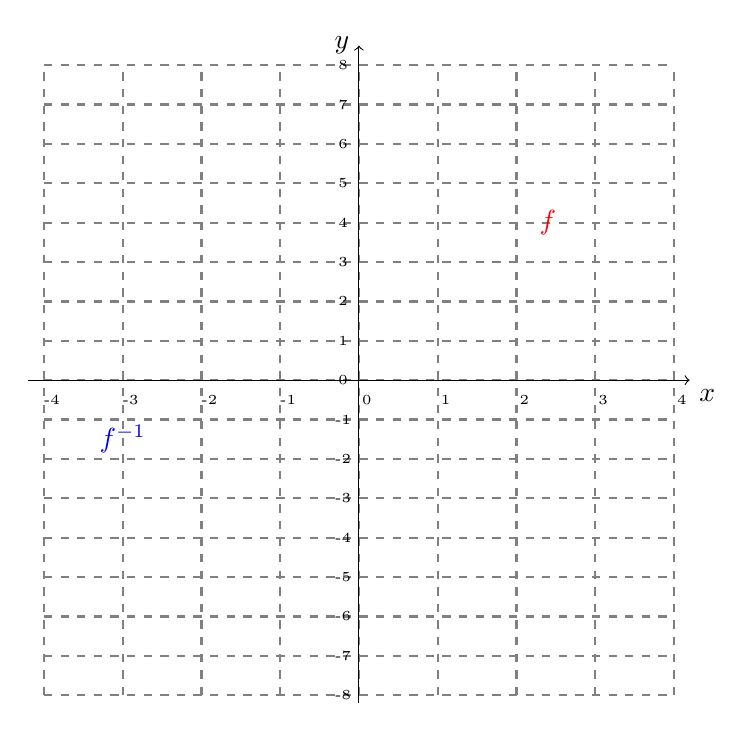
\begin{tikzpicture}[yscale=0.50,xscale=1.00] % Set the scale in both directions.
\draw[thick,color=gray,step=1.0, dashed] (-4.0,-8.0) grid (4,8); % draw the grid
                                             % from (0,-10) to (4,5).
\draw[->] (-4.2,0) -- (4.2,0) node[below right] {$x$}; % draw the line and
                                             % arrow to indicate the x-axis.
\draw[->] (0,-8.2) -- (0,8.5) node[left] {$y$}; % draw the line and
                                             % arrow to indicate the y-axis.
\draw[thick,color=red] plot[id=f,domain=-3.2:3.2, range=-10:10] function{2 * tan(x/2)}; %
                                             % A small change of domain can
                                             % result in a TeX capacity exceed
                                             % error. Just trial and error to
                                             % find a suitable domain.
\draw[thick,color=blue] plot[id=h,domain=-4:4] function{2 * atan(x/2)};
% \draw[thick,color=blue] plot[id=i,domain=2:2.934] function{5-1/(3-x)};
\draw(2.4,4) node[thick,color=red]{$f
$}; % Put the label somewhere
\draw(-3,-1.5) node[thick,color=blue]{$f^{-1}$}; % Put the label somewhere
% \draw(3.05,-4.5) node[thick,color=blue]{$i$}; % Put the label somewhere
% x-as
\draw(-3.9,-0.5) node[color=black]{{\tiny -4}};
\draw(-2.9,-0.5) node[color=black]{{\tiny -3}};
\draw(-1.9,-0.5) node[color=black]{{\tiny -2}};
\draw(-0.9,-0.5) node[color=black]{{\tiny -1}};
\draw(0.1,-0.5) node[color=black]{{\tiny 0}};
\draw(1.1,-0.5) node[color=black]{{\tiny 1}};
\draw(2.1,-0.5) node[color=black]{{\tiny 2}};
\draw(3.1,-0.5) node[color=black]{{\tiny 3}};
\draw(4.1,-0.5) node[color=black]{{\tiny 4}};
% y-as
\draw(-0.2,0) node[color=black]{{\tiny 0}};
\draw(-0.2,1) node[color=black]{{\tiny 1}};
\draw(-0.2,2) node[color=black]{{\tiny 2}};
\draw(-0.2,3) node[color=black]{{\tiny 3}};
\draw(-0.2,4) node[color=black]{{\tiny 4}};
\draw(-0.2,5) node[color=black]{{\tiny 5}};
\draw(-0.2,6) node[color=black]{{\tiny 6}};
\draw(-0.2,7) node[color=black]{{\tiny 7}};
\draw(-0.2,8) node[color=black]{{\tiny 8}};
\draw(-0.2,-1) node[color=black]{{\tiny -1}};
\draw(-0.2,-2) node[color=black]{{\tiny -2}};
\draw(-0.2,-3) node[color=black]{{\tiny -3}};
\draw(-0.2,-4) node[color=black]{{\tiny -4}};
\draw(-0.2,-5) node[color=black]{{\tiny -5}};
\draw(-0.2,-6) node[color=black]{{\tiny -6}};
\draw(-0.2,-7) node[color=black]{{\tiny -7}};
\draw(-0.2,-8) node[color=black]{{\tiny -8}};
\end{tikzpicture}
\end{center}
% If this method doesn't work because you don't have \texttt{gnuplot} then
% it might be wise to include a picture of your graph(s)
}


\exerciseenum{11}{%
\item%a
We follow the hint.
Suppose there exists a function $f:S\to \power{S}$ that is onto.
Now let $T = \setbuild{s\in S}{s\not\in f(s)}$.
Then $T\in \power{S}$, because T is a subset of S which contains all $s \in S$ for which $s \notin f(s)$.
We are going to show that there cannot be an element $t\in S$ such that
$f(t)=T$, which implies that $f$ is not onto, which is a contradiction.

\smallskip
Our definition of T states that if $t \in T$, then $t \notin f(t)$. This means that $T \neq f(t)$ which shows that the statement is false.
We can also prove this the other way. If $t \in f(t)$, then $t \notin T$.
\item%b
In a we saw that doesn't exists an onto function $S \rightarrow \power{S}$. This means that there exists at least one $x \in \power{S}$ for which holds that $x \notin S$. This means that $|S|$ is at least one lower than $|\power{S}|$, since only $\power{S}$ contains x. This shows that $|S| < |\power{S}|$ holds.
}

\end{document}
